\section{Introduction: 1D String}
\subsection{Newtonian Derivation}
Now let us consider the motion of 1D wave on a very long string.
\begin{itemize}
  \item Tension: $T$
  \item Line density (mass per unit length): $\mu$
\end{itemize}
Notice, that any point on the string is not moving in $x$ direction, otherwise the string itself will be moving.
Also, if we produce a "uniform" wave, then at all points on the string, the wave will have the same amplitude $A$ , wavelength $\lambda$, and frequency $f$  and velocity $v$.
\begin{figure}[htbp]
  \centering
  \begin{tikzpicture}[scale=1.0]
    \def\A{2.0}
    \def\ymax{\A*1.2}
    \def\ymin{-\A*1.2}
    \def\k{2}
    \def\xmax{2*pi*\k}

    % Draw the axes
    \draw[very thick, ->] (0,0) -- (\xmax+0.1,0) node[right] {$x$};
    \draw[very thick, ->] (0,\ymin) -- (0,\ymax) node[above] {$y$};

    % Draw the wave
    \draw[blue, thick] plot[domain=0:\xmax, samples=\samples] (\x,{\A * sin(\k*\x r)});

    % Add a legend
    \draw[blue, thick] (\xmax-1.5,\ymax+0.5) -- (\xmax-1,\ymax+0.5) node[right, black] {Wave: $y = \psi(x, t)$};
    \draw[thick, ->] (\xmax*0.45, \ymax+0.5) --(\xmax*0.55, \ymax+0.5) node[above, midway, black] {$v$};
  \end{tikzpicture}
  \caption{A plot of 1D wave on a string}
  \label{fig:string}
\end{figure}
This means that we can choose convinient point on the string, and calculate $A$, $\lambda$, $f$, and $v$, then the same values will be valid for all points on the string.
For a moving wave, a stationary point of view is not very useful, so we will use a moving point of view: the Lagrange description in fluid mechanics.

Consider moving in the $x$ direction, at the same constatn velocity $v$, as the wave.
Then, our new $x$ coordinate is given by the Galilean transformation:
\begin{align}
  \xi(x, t) & = x - vt
\end{align}
In this new perspective, we do not have to worry about the motion of the wave, since we are moving with the wave.
In short, the wave is stationary in the new coordinate system.
This means that vertical displacement of the wave at a point $\xi$ only depends on the $\xi$ coordinate, and not on time:
\begin{align}
  \psi(x, t) & = \psi(\xi)
\end{align}
and any point on the string seems to move at velocity $-v$.

Then immidiately,
\begin{align}
  \pdv{\psi(\xi)}{x}                    & = \pdv{\psi(\xi)}{\xi} \pdv{\xi}{x} = \pdv{\psi(\xi)}{\xi},                          \\
  \pdv{\psi(\xi)}{t}                    & = \pdv{\psi(\xi)}{\xi} \pdv{\xi}{t} = -v \pdv{\psi(\xi)}{\xi}                        \\
  \implies \quad \pdv[2]{\psi(\xi)}{x}  & = \pdv[2]{\psi(\xi)}{\xi}, \quad \pdv[2]{\psi(\xi)}{t} = v^2 \pdv[2]{\psi(\xi)}{\xi} \\
  \implies \quad \pdv[2]{\psi(x, t)}{x} & = \frac{1}{v^2} \pdv[2]{\psi(x, t)}{t}
\end{align}
we obtain the wave equation, but we should find its physical meaning.

\thm{Wave Equation in 1D}{
  The wave equation in 1D is given by:
  \begin{align}
    \pdv[2]{\psi(x, t)}{x} & = \frac{1}{v^2} \pdv[2]{\psi(x, t)}{t}
  \end{align}
  where $\psi(x, t)$ is the vertical displacement of the wave at point $x$ and time $t$, and $v$ is the velocity of the wave.
}


Now, let us focus on one of the peaks of the wave, at the point $\xi_0$.
\begin{figure}[htbp]
  \centering
  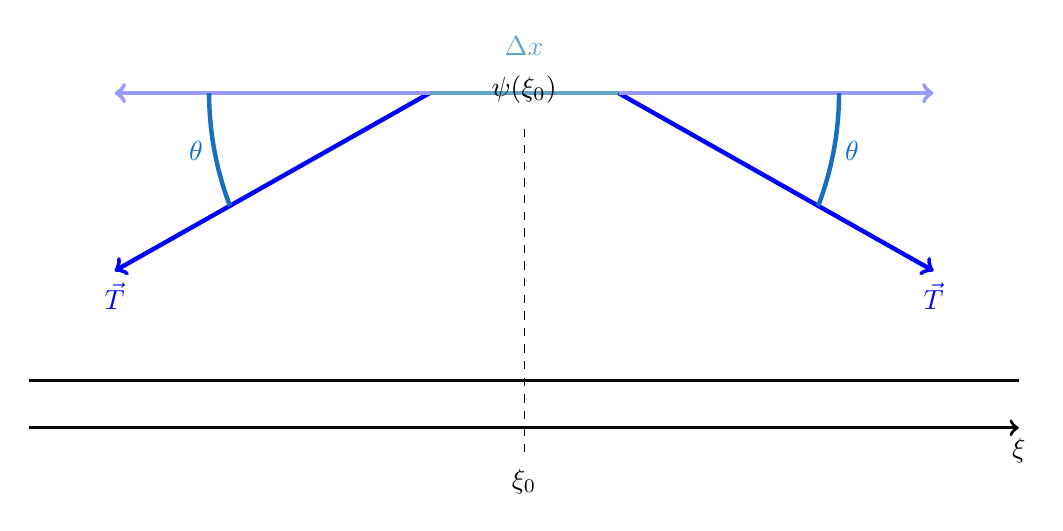
\begin{tikzpicture}[scale=2.0]
    \def\dx{2.0}
    \def\c{cos(0.6 r)}
    \def\a{sin(0.6 r)}
    \def\b{\c + \a * \dx}

    \draw[very thick, ->] (-pi, -1.3) -- (pi, -1.3) node [below] {$\xi$};
    \draw[dashed] (0, 0.6) -- (0, -1.5) node [below] {$\xi_0$};

    \draw[black, very thick] plot[domain=-pi:pi, samples=\samples] (\x,{cos(\x r)});
    \draw[cyan!50!gray, ultra thick] plot[domain=-0.6:0.6, samples=\samples] (\x,{cos(\x r)});
    \draw[cyan!50!gray] (0, 1) node[above] {$\Delta x$};
    \draw[ultra thick, blue, ->] (0.6,{\c}) -- (0.6 + \dx, {\c - \a * \dx}) node [below] {$\vec{T}$};
    \draw[ultra thick, blue, ->] (-0.6, {\c}) -- (-0.6 - \dx, {\c -  \a * \dx}) node [below] {$\vec{T}$};
    \draw[ultra thick, blue!40!white, ->] (0.6,{\c}) -- (0.6 + \dx, {\c});
    \draw[ultra thick, blue!40!white, ->] (-0.6, {\c}) -- (-0.6 - \dx, {\c});
    \draw[ultra thick, cyan!50!blue] (0.6 + 0.7 * \dx, {\c}) arc [start angle=0, end angle = -21, radius = \dx] node[midway,right] {$\theta$};
    \draw[ultra thick, cyan!50!blue] (-0.6 - 0.7 * \dx, {\c}) arc [start angle=180, end angle = 180 + 21, radius = \dx] node[midway,left] {$\theta$};
    \draw (0, 1) node [below] {$\psi(\xi_0)$};
  \end{tikzpicture}
  \caption{A peak of the wave}
  \label{fig:wave_peak}
\end{figure}
The tension on the string at $\xi_0$ cancels out horizontally, but adds vertically:
\begin{align}
  F_x & = T \cos \theta - T \cos \theta = 0                                                                                     \\
  F_y & = F_{-y} + F_{+y} = - T \pdif{x} \psi\pab{\xi_0 + \frac{\Delta x}{2}} + T \pdif{x} \psi\pab{\xi_0 + \frac{\Delta x}{2}}
\end{align}
Thus the equation of motion for the infinitisimal segment of the string at $\xi_0$ is given by:
\begin{align}
  \vec{F} & = m \ddot{\vec{r}} \iff T \pab{\pdif{x} \psi\pab{\xi_0 + \frac{\Delta x}{2}} - \pdif{x} \psi\pab{\xi_0 - \frac{\Delta x}{2}}} = \mu \Delta x \pdif{t}^2 \psi(\xi_0)
\end{align}
by rearranging,
\begin{align}
  \frac{1}{\Delta x} \pab{\pdif{x} \psi\pab{\xi_0 + \frac{\Delta x}{2}} - \pdif{x} \psi\pab{\xi_0 - \frac{\Delta x}{2}}}
   & = \frac{\mu}{T} \pdif{t}^2 \psi(\xi_0)
\end{align}
as $\Delta x \to 0$, LHS becomes the derivative of the first derivative:
\begin{align}
  \pdif[2]{x} \psi(\xi_0) & = \frac{\mu}{T} \pdif[2]{t} \psi(\xi_0)
\end{align}
Now, note that the infinitisimal section experiences force in $y$ direction, while it moves in $x$ direction,
This is equivalent to a circular motion with radius $r = \psi(\xi_0)$:
\begin{align}
  F_c & = \frac{mv^2}{r} = \frac{\mu \Delta x v^2}{\psi(\xi_0)} = F_y
\end{align}
In this limit of $\Delta x \to 0$, $\Delta x = 2 \psi(\xi_0) \theta$,
\begin{align}
  \implies \quad 2 \theta \mu v^2 & = 2 T \sin \theta \approx 2 T \theta \\
  \implies \quad v^2              & = \frac{T}{\mu}
\end{align}
Thus, the wave equation can be written as:
\begin{align}
  \pdv[2]{\psi(x, t)}{x} & = \frac{1}{v^2} \pdv[2]{\psi(x, t)}{t}, \quad \text{where } v = \sqrt{\frac{T}{\mu}}
\end{align}



